\documentclass{article}

\usepackage{simcmag}
\usepackage[export]{adjustbox}

\date{\hspace{30mm}}
\currentvolume{4}

\newcommand{\simcmagcredits}{
  \footnotesize
  \begin{tcolorbox}[boxrule=1.0pt,colback=white,hbox,before upper*=\begin{tabular}{l},after upper*=\end{tabular}, sharp corners,left=-5pt,right=-5pt]
  Editor-in-Chief: Edward Y. \\
  Editor: Cecilia S. \\
  Staff Writers:\\
  \begin{tabular}{ll}
    Cecilia S. & Edward Y. \\
    Joyce H. & Michael Y.\\
    Owen X. & Rohan D. \\
    William Y. F. & William G. 
  \end{tabular}
  \end{tcolorbox}
}

% uasage of picinpar:
%\begin{window}[1,l,\includegraphics{},caption]xxxxx\end{window}

% usage of window:
% \begin{window}[2,r,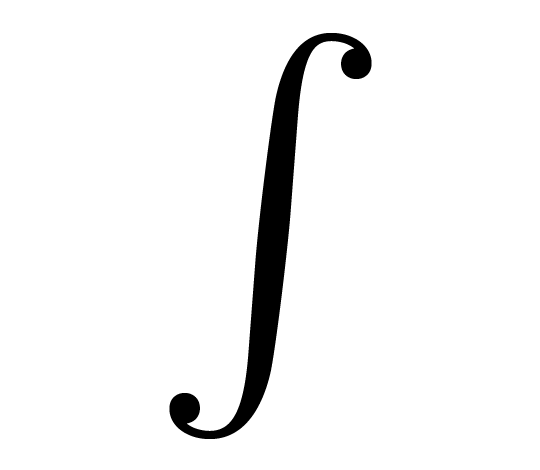
\includegraphics[width=1.0in]{img/logo.png},\centerline{a picture}]
% Duis aute irure dolor in reprehenderit in voluptate velit esse cillum dolore eu fugiat nulla pariatur. Excepteur sint occaecat cupidatat non proident, sunt in culpa qui officia deserunt mollit anim id est laborum
% \end{window}

%%%%%%%%%  Front matter   %%%%%%%%%
\begin{document}
\maketitle
\begin{minipage}[t]{.45\textwidth}\thispagestyle{empty}
  \vspace{-11mm}
  \tableofcontents
\end{minipage}% 
\begin{minipage}[t]{.1\textwidth}\thispagestyle{empty}
  \;
\end{minipage}% 
\begin{minipage}[t]{.45\textwidth}\thispagestyle{empty}
  \footnotesize
  \setlength{\parskip}{5pt}
  \vspace{-7mm}
  {\itshape
    \begin{center}
        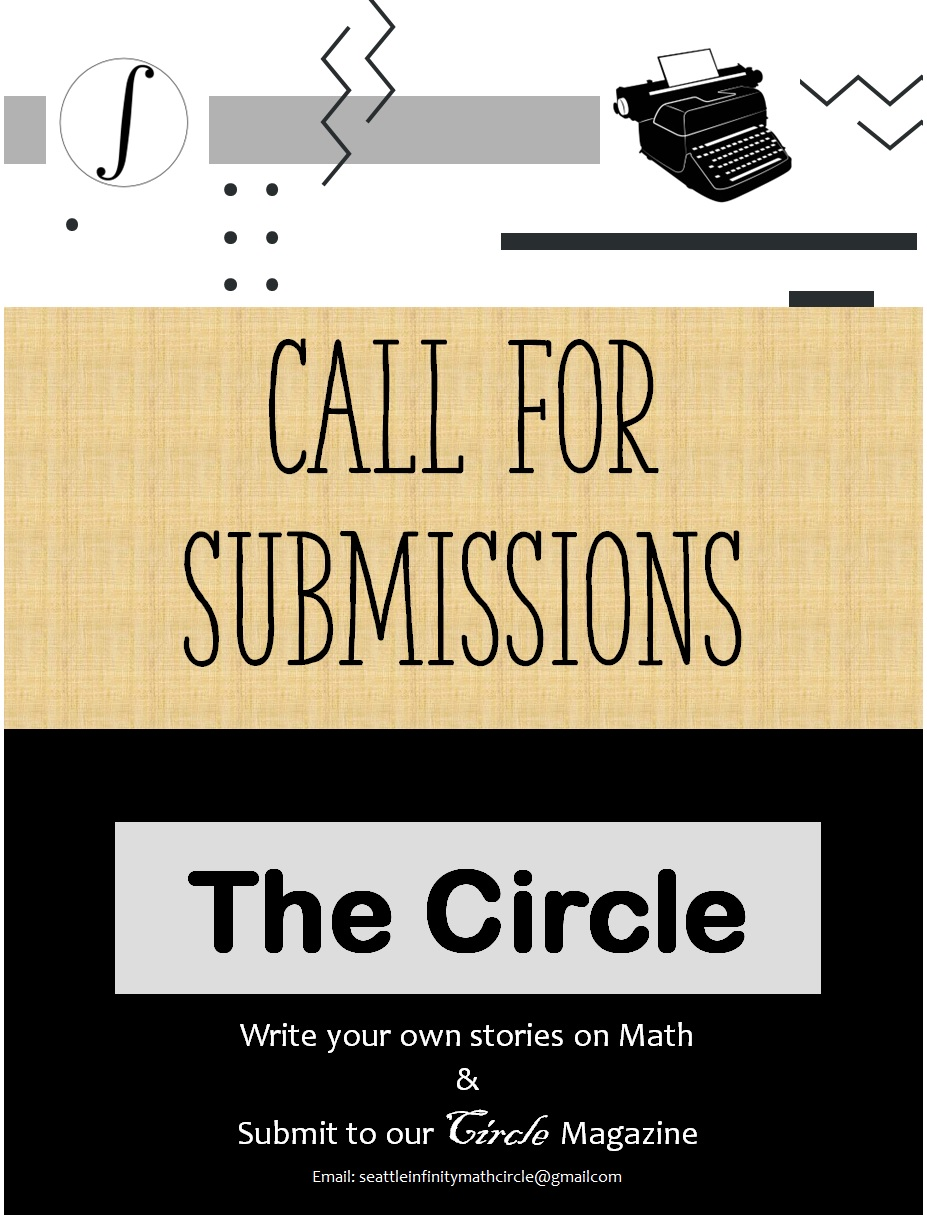
\includegraphics[scale=0.45]{Magazines/img/Vol4/call4submission.jpg}
        \\
    \href{https://docs.google.com/forms/d/e/1FAIpQLSdqg6k7R5THXqhu7dHN6RjT4ynvVppoQ0uZdLo0cbu5E4VPZQ/viewform}{Submit an article to the Circle here!}
    \end{center}    
}
\end{minipage}

\vspace{3mm}


\begin{multicols}{3}

\articletitle{Axiomatic Math}{William Gvozdjak}{}
\begin{center}
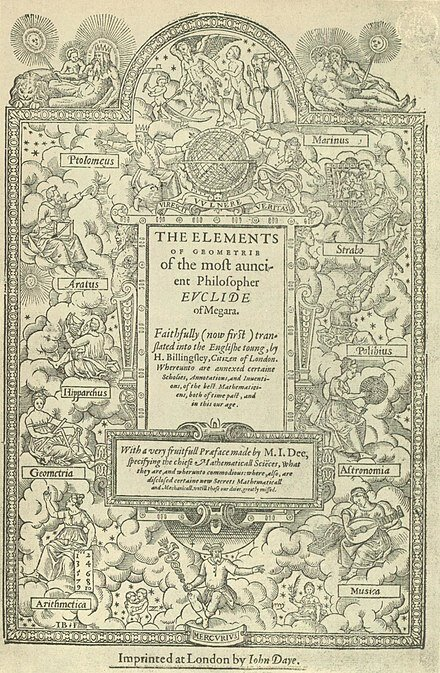
\includegraphics[scale=0.25]{Magazines/img/Vol4/euclid_elements.jpg}
\end{center}
You may have heard of the word \textit{axiom} before in the context of math. Whether through the axioms for geometry that Euclid came up with or the article \textit{Axiom of Choice} in \textit{The Circle Volume 1}, axioms are a crucial component of mathematics. But the most crucial question often eludes us until we reach college classes: what even are axioms?

To demonstrate this, we'll start with an example: linear algebra. Key to the field of linear algebra is a \textbf{vector}: a line segment starting at one point and ending at another. What defines a vector is its magnitude (its length) and its direction. Two vectors are considered equal if and only if they have equal magnitude and direction. For example, the following two vectors are equal:

\begin{center}
    \begin{asy}
        unitsize(1cm);
        draw((0, 0)--(1, 0.5), EndArrow);
        draw((1.25, 0)--(2.25, 0.5), EndArrow);
    \end{asy}
\end{center}

but these two are not:
\begin{center}
    \begin{asy}
        unitsize(1cm);
        draw((0, 0)--(1, 0.5), EndArrow);
        draw((1.75, 0)--(1.25, 0.75), EndArrow);
    \end{asy}
\end{center}

Let's suppose that the set of all 2-dimensional vectors is called $\mathbf{V}$. Then, we define the following concepts:

\begin{enumerate}
    \item \textbf{Vector addition}. If $\mathbf{v}$ and $\mathbf{w}$ are two vectors in $\mathbf{V}$, then we define $\mathbf{v}+\mathbf{w}$ as follows: place $\mathbf{w}$ so that its tail as at the tip of $\mathbf{v}$. Then $\mathbf{v}+\mathbf{w}$ is the vector with tail at the tail of $\mathbf{v}$, and tip at the tip of $\mathbf{w}$.

    \begin{center}
        \begin{asy}
            unitsize(1cm);
            draw((0, 0)--(1, 0.5), EndArrow);
            draw((1, 0.5)--(1.25, 1), EndArrow);
            draw((0, 0)--(1.25, 1), red, EndArrow);
            label("$\mathbf{v}$", (0, 0)--(1, 0.5), dir(300));
            label("$\mathbf{w}$", (1, 0.5)--(1.25, 1), dir(-30));
            label("$\mathbf{v}+\mathbf{w}$", (0, 0)--(1.25, 1), dir(130));
        \end{asy}
    \end{center}

    \item \textbf{Scalar multiplication}. If $\mathbf{v}$ is a vector in $\mathbf{V}$ and $a$ is a real number, then $a\mathbf{v}$ is the vector with magnitude $a$ times the magnitude of $\mathbf{v}$ and the same direction as $\mathbf{v}$.

    \begin{center}
        \begin{asy}
            unitsize(1cm);
            draw((0, 0)--(1, 0.5), EndArrow);
            draw((1.25, 0)--(3.25, 1), EndArrow);

            label("$\mathbf{v}$", (0, 0)--(1, 0.5), dir(130));
            label("$2\mathbf{v}$", (1.25, 0)--(3.25, 1), dir(130));
        \end{asy}
    \end{center}

    \item \textbf{Zero vector}. We define the zero vector $\mathbf{0}$ of $\mathbf{V}$ to be a vector with magnitude $0$.
\end{enumerate}

Now, we observe the following properties, where $\mathbf{u}$, $\mathbf{v}$, and $\mathbf{w}$ are two vectors in $\mathbf{V}$.

\begin{enumerate}
    \item $a\mathbf{v}\in\mathbf{V}$, $\mathbf{v}+\mathbf{w}\in\mathbf{V}$. Formally, we say that $\mathbf{V}$ is \textbf{closed} under vector addition and scalar multiplication. This is obvious: the operations we defined above result in elements of $\mathbf{V}$.
    \item $\mathbf{v}+\mathbf{w}=\mathbf{w}+\mathbf{v}$ (vectors in $\mathbf{V}$ are \textbf{commutative}). Verify this using the definition of vector addition above!
    \item $(\mathbf{u}+\mathbf{v})+\mathbf{w}=\mathbf{u}+(\mathbf{v}+\mathbf{w})$ (vectors in $\mathbf{V}$ are \textbf{associative}).
    \item $\mathbf{v}+\mathbf{0}=\mathbf{v}$ ($\mathbf{0}$ is the \textbf{additive identity} of $\mathbf{V}$).
    \item $0\mathbf{v}=\mathbf{0}$.
    \item $1\mathbf{v}=\mathbf{v}$ ($1$ is the \textbf{multiplicative identity}).
    \item $a(b\mathbf{v})=(ab)\mathbf{v}$.
    \item $a(\mathbf{v}+\mathbf{w})=a\mathbf{v}+a\mathbf{w}$ (scalar multiplication is \textbf{distributive} over vector addition).
    \item $(a+b)\mathbf{v}=a\mathbf{v}+b\mathbf{v}$.
\end{enumerate}

Now, we introduce the crucial step: \textbf{abstracting away} from these types of vectors. In other words, instead of \textit{observing} the above 9 properties from vectors, we will \textit{assume} that the properties are true, and look at what potential objects satisfy these properties. Each ``type'' of object that does satisfy these properties forms a \textbf{vector space}.

Formally, a vector space $\mathbf{V}$ is a set of objects known as \textit{vectors} (notice that these vectors may or may not be the same vectors as before! The entire point of defining a vector space is to create a sort of template for a generic set of objects). For these objects, two types of operations must be defined: scalar multiplication $a\mathbf{v}$ and vector addition $\mathbf{v}+\mathbf{w}$. The zero vector $\mathbf{0}$ must exist. Then, for all vectors $\mathbf{u}$, $\mathbf{v}$, and $\mathbf{w}$ in $\mathbf{V}$ and all real numbers $a$ and $b$, the following properties must be true:

\begin{enumerate}
    \item $a\mathbf{v}\in\mathbf{V}$, $\mathbf{v}+\mathbf{w}\in\mathbf{V}$

    \item $\mathbf{v}+\mathbf{w}=\mathbf{w}+\mathbf{v}$

    \item $(\mathbf{u}+\mathbf{v})+\mathbf{w}=\mathbf{u}+(\mathbf{v}+\mathbf{w})$

    \item $\mathbf{v}+\mathbf{0}=\mathbf{v}$

    \item $0\mathbf{v}=\mathbf{0}$.

    \item $1\mathbf{v}=\mathbf{v}$

    \item $a(b\mathbf{v})=(ab)\mathbf{v}$.

    \item $a(\mathbf{v}+\mathbf{w})=a\mathbf{v}+a\mathbf{w}$

    \item $(a+b)\mathbf{v}=a\mathbf{v}+b\mathbf{v}$.
\end{enumerate}

These 9 properties are known as \textbf{axioms} (in this special case, they're known as the \textbf{axioms of vector spaces}): they are certain requirements that must be met in order for something to be called a vector space. Notice that the set of two-dimensional vectors that we discussed earlier forms a vector space, as they satisfy all of the above axioms. There exist many other vector spaces as well: function spaces, polynomial spaces, and much more.

So, why do we care? The answer is: using these measly 9 axioms, it turns out that we can prove many interesting properties about vector spaces. Just by satisfying these axioms, we can infer fascinating ideas about a set of objects, which we can use to explore and better understand them.

Axioms are not just used in linear algebra: they're used almost everywhere, from group theory to geometry. So be sure to take a moment and appreciate the significance of axioms in the field you're exploring the next time you encounter a mathematical topic.

\begin{center}
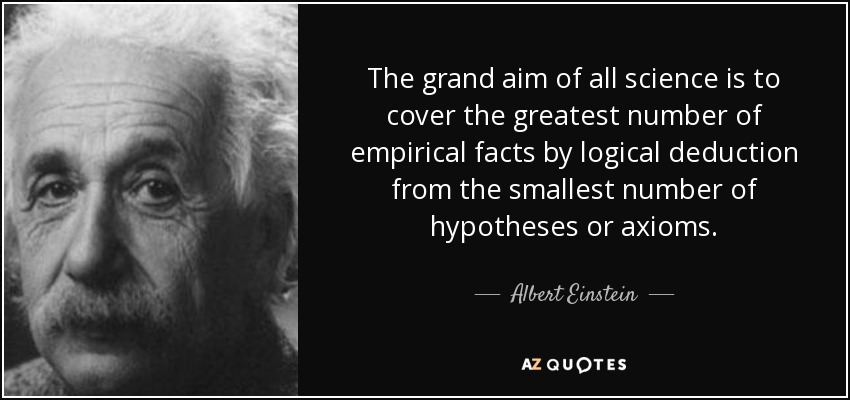
\includegraphics[scale=0.18]{Magazines/img/Vol4/albert_einstein_quote.jpg}
\end{center}
\closearticle

\articletitle{But What is Vieta Jumping?}{Rohan Dhillon}{}
1988. The IMO problem selection committee has just finished choosing problems for that years test. Nothing too out of the ordinary...except for problem 6: one of the few problems that the selection committee couldn't solve in 6 hours. Even after sending the problem to Australia's top number theorists, a solution eluded them. Nonetheless, the problem was put on the test. And there were 11 7s. How? What technique did they use?

Like most number theory problems, the statement seems simple: \textit{If a, b are positive integers such that $ab+1 $ divides $a^2+b^2,$ show that $\frac{a^2+b^2}{ab+1}$ is a perfect square.} 

\textit{Huh. Doesn't seem too bad--maybe take a few mods?} Nope. Indeed to solve this problem, we have to combine the nimbleness of number theory with the heavy machinery of algebra. 

But I'm getting ahead of myself--motivation first, solution second. If we were to use traditional techniques, we would have 3 variables (by setting the fraction equal to some perfect square $z^2$) and no constants, giving us little guidance on what to choose as a modulo. So a direct proof is probably going to be quite difficult, hence we try proof by contradiction, and in particular, we try infinite descent since we can't use modular contradictions easily.

Let $\frac{a^2+b^2}{ab+1}=z,$ where z is not a perfect square. Then suppose we have $a,b$ such that $a^2+b^2=abz+z.$ Suppose that $a_0$ and $b_0$ are the integers satisfying this constraint such that $a_0+b_0$ (we have to quantify this notion of the "smallest" positive integers when we're using two or more integers in infinite descent). Since we can't see much else, we try moving everything to one side of the equation in the hopes of...\textit{something} happening.

So $a_0^2-a_0b_0z+b_0^2-z=0.$ Hmm, a quadratic equation? You know what, sure--we don't have much time left. Set $a_0$ to $x$ for the ease of our eyes to get $x^2-(b_0z)x+b_0^2-z=0.$ Well, we know that $a_0$ is one root of this equation, and we're looking for infinite descent so what if the other root is smaller? By Vieta's, the other root $a_1$ satisfies $a_1=b_0z-a_0$ and $a_1=\frac{b_0^2-z}{a_0}.$

The first constraint shows that $a_1$ is an integer, but we need to show that it's a \textit{positive} integer. But that's where our second equation comes in: it even kills two constraints with one(ish) inequality! We can quickly note that $a_1 \ne 0$ since $z$ is not a perfect square, and we also have that $\frac{a_1^2+b_0^2}{a_1b_0+1}=z > 0,$ thus $a_1b_0 > -1$ and since $a_1, b_0$ are both integers (and thus their product is as well), we have $a_1$ is a positive integer. 

So now we have found a different solution from our starting pair $(a_0,b_0)$ but we have to show that $a_1+b_0 < a_0+b_0$ which is equivalent to showing that $a_1<a_0.$ From our first equation, this is tantamount to showing $b_0z<2a_0,$ which I'll leave you to do! (Ah, proof by exercise to the reader--great tool right?)

\begin{center}
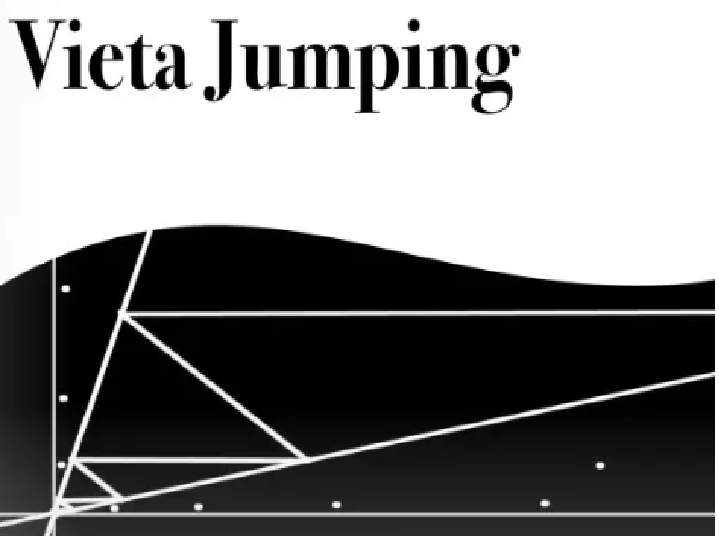
\includegraphics[scale=0.5]{Magazines/img/Vol4/vieta_jumping.png}
\end{center}

Vieta jumping is, however, more than just a cool way to solve olympiad problems--it also offers us a glimpse into the inner working of algebraic number theory and the interconnectedness of mathematics. There is no "purely" geometric or algebraic problem, rather every problem can fall in every category. (Indeed, the problem we did can also be about finding hyberbolas in the Cartesian Plane--see if you can reframe it to see why!)
\closearticle

\articletitle{The Euclidean Algorithm}{William Y. Feng}{}

The \textit{greatest common divisor} (gcd) of two integers $a$ and $b$, written $\gcd(a, b)$, is defined as the greatest positive integer that divides both $a$ and $b$.

For example, the gcd of 54 and 30 is 6, because 6 divides both 54 and 30, while no larger integer has this property.

The greatest common divisor operation is a familiar operation to number theorists. In a theoretical setting, mathematicians rarely have to find the greatest common divisor of two cold hard numbers. But we're not going to talk about vague, general things here! We're going to find out how to actually compute the gcd of any two given numbers.

\textbf{A special property of the gcd:} We know that 6 divides both 54 and 30. Notice how 6 also divides their difference: $54 - 30 = 24$. 6 also divides their \textit{sum}, $54 + 30 = 84$. This fact holds in general: if an integer $n$ is a divisor of both $a$ and $b$, then it divides $a - b$ and $a + b$ as well.

Coincidentally, this holds for the gcd too:

\textbf{Big Claim.} If $n$ is the greatest common divisor of $a$ and $b$, then $n$ is also the greatest common divisor of $b$ and $a - b$.

To see why this is true, assume otherwise; perhaps there exists a larger number $d$ that divides both $b$ and $a - b$. But then, according to our facts above, $d$ would divide $b + (a - b) = a$ too, contradicting our assumption that 6 was the \textit{greatest} common divisor of $a$ and $b$.

Now, let's put this to use and find the greatest common divisor of 49 and 63. Maybe it's already obvious to you what the answer is, but play along! Again, this is the largest positive integer that is a divisor of both 49 and 63. Let this number be $d$.

One thing we certainly \textit{don't} want to do is test a bunch of numbers and determine the largest one that divides both 49 and 63. What we can do instead is apply the Big Claim: we know that $d$ should also be the greatest common divisor of 49 and the \textit{difference} between 49 and 63,
$$63 - 49 = 14.$$
So now we have reduced the problem to finding the greatest common divisor of 49 and \textit{14}. In other words, we
$$\gcd(49, 63) = \gcd(49, 14).$$
This seems good; we've essentially gotten rid of a big number, 63, and replaced it with a smaller number, 14.

To find $\gcd(49, 14)$, we can apply the Big Claim again! This time, we subtract 14 from 49 to get 35:
$$\gcd(49, 14) = \gcd(35, 14).$$
We can do it again, subtracting 14 from 35:
$$\gcd(35, 14) = \gcd(21, 14)$$
and again:
$$\gcd(21, 14) = \gcd(7, 14).$$
Now we subtract 7 from 14 to get
$$\gcd(7, 14) = \gcd(7, 7),$$
and then one last time to get
$$\gcd(7, 7) = \gcd(7, 0).$$
The greatest common divisor of zero and another number is always the other number, because everything divides zero. Thus, $\gcd(7, 0) = 7$. Condensing all our steps, we see that we went from
$$\gcd(49, 63) = \gcd(7, 0) = 7,$$
solely by applying the Big Claim. And we see that throughout all our reductions, 7 remained the greatest common divisor of both number.

\begin{center}
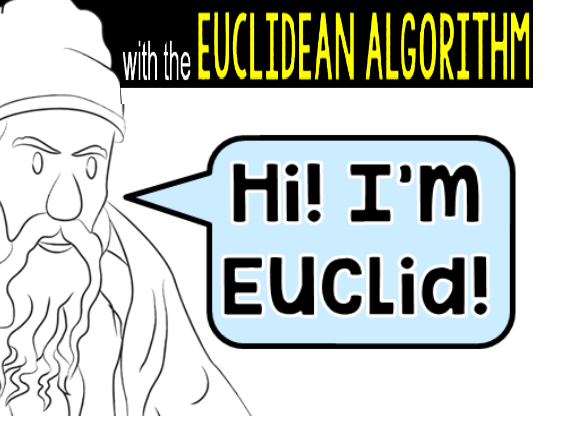
\includegraphics[scale=0.7]{Magazines/img/Vol4/euclidean.png}
\end{center}

This is the process behind the \textbf{Euclidean Algorithm}: To find the gcd of $a$ and $b$, we can subtract the smaller number from the larger number to reduce the overall size of the two numbers. From there, we rinse and repeat until we get down to sufficiently small numbers to determine the answer directly.

\textbf{A small problem:} Suppose we're trying to find the gcd of 15174 and 702. The answer isn't immediately obvious, so we try the subtraction trick by turning 15174 into $15174 - 702 = 14472$. We get
$$\gcd(702, 15174) = \gcd(702, 14472).$$
Still not obvious what the answer is, so let's try again, this time replacing $14472$ with $14472 - 702 = 13770$:
$$\gcd(702, 14472) = \gcd(702, 13370).$$
If we keep doing this---subtracting 702 from the second number---we'll eventually get down to
\begin{align*}
\gcd(702, 1134) & = \gcd(702, 1134 - 702) \\
    & = \gcd(702, 432)
\end{align*}

This livens things up a bit and now we can instead subtract 432 from 702. But was there a better way to get here? Let's look at the original query:
$$\gcd(702, 15174)$$
Evidently we'll be subtracting 702 from the second number for a while. Instead of doing all these subtractions, we can just do them all at once and \textit{take the remainder} with 15174 by 702. Perhaps this is best illustrated by calculating the quotient and remainder:
$$15174 = 21(702) + 432.$$
Essentially, we'll subtract 702 from the first number a whopping \textit{21 times} before the first number becomes 432 and we can start subtracting from 702 instead. In this case, 432 is the \textit{remainder} when 15174 is divided by 702.

In general, if we want o find $\gcd(a, b)$ and $b$ is smaller than $a$, then we know that this gcd equals $\gcd(a\,\%\,b, b)$, where $a\,\%\,b$ denotes the remainder when $a$ is divided by $b$. If we apply \textit{this} until we get one of the arguments down to zero, we get \textit{54} as the gcd of 702 and 15174.

\textbf{Summary:} Putting it all together, we get the following algorithm:
\begin{enumerate}
\item Take two numbers, $a$ and $b$. Possibly reorder them so that $a < b$.
\item Subtract the smaller number from the larger one as much as possible (using the remainder operation to speed things up).
\item Once one of the numbers becomes 0, the other number is the gcd.
\end{enumerate}
The Euclidean Algorithm has many applications in algorithmic number theory—one of them involves extending the algorithm to find \textit{modular inverses}, a critical component in cryptographic protocols such as the \textit{Diffie-Hellman key exchange} and the \textit{RSA} encryption scheme.
\begin{center}
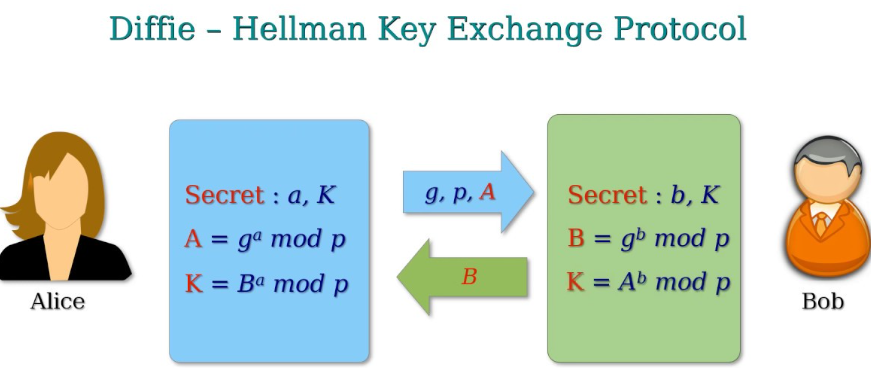
\includegraphics[scale=0.4]{Magazines/img/Vol4/diffie_hellman.png}
\end{center}
\closearticle


\articletitle{A Common Yet Unknown Problem-Solving Technique: States}{William Gvozdjak}{}
Take a moment to read the following problem:

``I'm flipping a fair coin repeatedly. I'll keep flipping it until I reach a sequence of 3 consecutive flips that are HT. On average, how many times will I flip the coin?''

At first glance, this problem seems really difficult: how are we supposed to find the average number of times that I'll flip the coin? In reality, if you know the right technique, this question becomes a simple problem of algebra.


First, we define each \textbf{state}: possible positions to be at in terms of the flips. Our first state, $1$, is the ``null'' state: there have been no flips that contribute to the desired HT. This is both at the start of the sequence of flips, and also at any time where the last flip was a T (this is because if the last flip was a T, we essentially are restarting, as we can't use that T to create an HT sequence). Then, we also have the state $2$, for when the last flip was an H. Notice that it doesn't matter what flips were prior to that H: the expected number of flips to reach HT will be the same no matter what flips were before that H. Finally, we have the state $3$, where the last two flips are HT: this is the desired state.

Now, define $a_i$ to be the expected number of flips to reach HT from the state $i$. First, note that we clearly have $a_3=0$: we're starting at the state HT, so we've already reached HT!

Consider state $2$ (we currently have H). There's a $\frac{1}{2}$ probability that we'll reach an HT from there (i.e., flip a T in the next flip). Therefore, we know that there's a $\frac{1}{2}$ probability that the expected number of flips to reach HT is $a_3+1$ (note that we must add $1$ to account for the one flip that we must use to reach state $3$). But there's also a $\frac{1}{2}$ probability that we flip an H in the next flip, which simply returns us to state $2$. Hence, we have
\[a_2=\frac{1}{2}(a_3+1)+\frac{1}{2}(a_2+1).\]
Finally, consider state $1$ (we currently either have nothing or T). If we flip an H, then we move to state $2$, and if we flip a T, we stay at state $1$. Therefore, we know that
\[a_1=\frac{1}{2}(a_2+1)+\frac{1}{2}(a_1+1).\]
Notice that we are looking for the value of $a_1$, as we want to find the expected number of flips necessary to reach HT from a state consisting of no flips.

We therefore have the following system of equations:
\begin{align*}
a_1&=\frac{1}{2}(a_2+1)+\frac{1}{2}(a_1+1) \\
a_2&=\frac{1}{2}(a_3+1)+\frac{1}{2}(a_2+1) \\
a_3&=0.
\end{align*}
But this is simply a system of $3$ linear equations with $3$ variables -- it's just an algebra problem! We can solve these three equations just as we would with any other system of linear equations, and we'd find that $a_1=\boxed{4}$.

\begin{center}
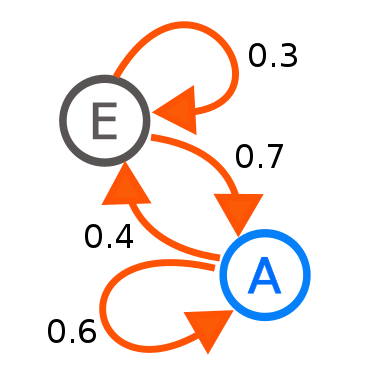
\includegraphics[scale=0.38]{Magazines/img/Vol4/finite_state.png}
\end{center}

In summary, states is a powerful technique that can be used to reduce seemingly difficult counting problems into matters of simple algebra and arithmetic. But also remember that this article just brushed the surface of states: states can be used to solve many different types of problems, from problems like the above one to walks on a grid. States are also an introduction to a more advanced topic known as \textbf{Markov chains} -- if you found this interesting, I highly recommend you explore and learn more about them!
\closearticle

\articletitle{Coin Change}{William Y. Feng}{}

 You just moved to the UK last week, and, needing to provide a living for yourself, you found a job as a cashier at a large retail store in central London. Today's your first day on the job—you're a little nervous, mostly about rude customers, but are excited to do the job nonetheless.

The first customer of the day walks to your checkout line and hands you a calculator. You scan it, run the totals, and it comes out to $\pounds 9.60$. The customer pays with a ten-pound note, so you'll need to give them back 40 pence in change.
\begin{center}
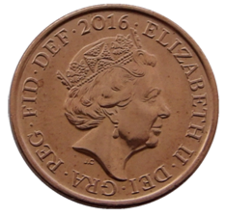
\includegraphics[scale=0.6]{Magazines/img/Vol4/british_coin.png}
\end{center}
Seems simple enough; the cash register pops open and you discover \textit{six coin denominations}: \textit{1p} \textit{p is short for pence}, \textit{2p}, \textit{5p}, \textit{10p}, \textit{20p}, and \textit{25p}.

Making 40 pence should be a breeze. You use a \textit{greedy algorithm} and start by taking a 25p coin, leaving 15p to make—so you finish with a 10p and a 5p. You collect these three coins and hand them to the customer.

"Wait," they say. "I'll excuse you, since I can tell you're probably an American and it looks like you're new on the job—but there's a more efficient way to make 40 pence."

You're confused. You just went through the coin denominations in decreasing order, and 25p, 10p, and 5p seems like a pretty optimal way to make 40p change.

"You could have just given me two 20p coins."

The realization hits you with the weight of a train. How did your greedy algorithm fail? Is using up large-denomination coins first not the optimal way to make change to minimize the number of coins? The customer's remark shakes the very foundations of your understanding of currency. Maybe you weren't made out to be a cashier in the UK after all.

\begin{center}
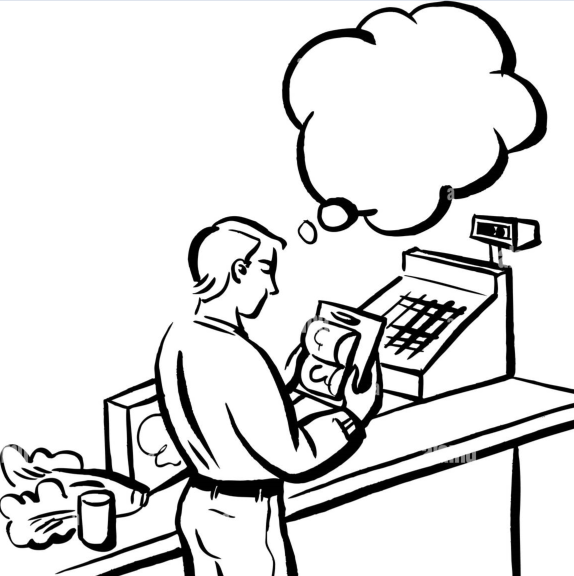
\includegraphics[scale=0.6]{Magazines/img/Vol4/cashier.jpg}
\end{center}

"It's okay, you don't get the same problem in America. And we don't usually get this in the UK either; we can prove that it's because of those commemorative 25p coins that your greedy algorithm didn't work."

This customer must be either a genius or a mathematician. You're interested in hearing more; perhaps this person can rebuild some of your foundations of mathematics that they just violently tore down.

"Here's a simpler example: suppose we have to make 10 pence with only 1-pence, 3-pence, and 4-pence coins. What's the minimum number of coins we must use?"

You're hesitant to reply, because this customer has just made you so unsure of yourself. The greedy approach would have you use as many 4p coins as possible first, then 3p coins, then 1p coins. This would result in using two 4p coins and two 1p coins to make 10p.

"Surely there's a more optimal way than being greedy here," you say. "I can use four coins—two 4p and two 1p—to make 10p, but we can probably do better."

"You're exactly right," says the customer. "Consider this: to make 10 pence, we have three options:
\begin{enumerate}
\item Take a 4p coin, and make the remaining 6p optimally
\item Take a 3p coin, and make the remaining 7p optimally
\item Take a 1p coin, and make the remaining 9p optimally
\end{enumerate}
In other words, if we define the following function:
$C(n) = \text{minimum number of coins to make n pence}$
then we can write
\[
C(n) = \text{minimum of }
\begin{cases}
    1 + C(n - 4) \\
    1 + C(n - 3) \\
    1 + C(n - 1)
\end{cases}
\]
Each of those three cases is one potential universe of possibilities, and we want the one which uses the minimum number of coins. This function only works in this specific scenario—we'd have to modify it if we wanted to use, say, British coin denominations."

"That's an interesting way of framing this problem. How can we actually compute $C(n)$, though?" you reply.

"Good question! We can do it by iteratively finding $C(i)$ for all the $i$ less than $n$. Suppose we want to calculate $C(10)$, and already have all the values of $C(1), C(2), \dots, C(9)$.

\begin{table}[h]
    \centering
    \begin{tabular}{c|c|c|c|c|c|c|c|c|c|c}
        $n$ & 1 & 2 & 3 & 4 & 5 & 6 & 7 & 8 & 9 & 10 \\\hline
        $C(n)$ & 1 & 2 & 1 & 1 & 2 & 2 & 2 & 2 & 3 & 
    \end{tabular}
\end{table}
To fill out the entry for $C(n)$, we consider each of those three possibilities.
\begin{enumerate}
    \item What if we used a 4p coin? Then we'd have 6p left, which we \textit{know for sure} is optimally constructed with $C(6) = 2$ coins. Adding on the 4p coin, this makes 3 coins in total.

    \item There are other ways—if we used a 3p coin, then we'd have 7p left, which we know can be optimally constructed with $C(7) = 2$ coins, giving the possibility to construct 10p with 3 coins yet again.

    \item And if we used a 1p coin, then we'd have 9p left, which we know is optimally constructible with $C(9) = 3$ coins, making 4 coins total.
\end{enumerate}

Thus we have three alternatives, and we take the best one. In this case, either of the first two work, so $C(10)$ should be 4. We could even keep going if we wanted to; now that we have the first 10 values of $C(n)$, we can find $C(11)$, then $C(12)$, and so on."

Fascinating! This customer has just given you an incredibly fast way to determine the minimum number of coins to make any arbitrary amount of change.

"And you said this works for British denominations, too?" you ask.

"Why, of course—the function would just look something like this instead:
\[
C(n) = \text{minimum of }
\begin{cases}
    1 + C(n - 25) \\
    1 + C(n - 20) \\
    1 + C(n - 10) \\
    1 + C(n - 5) \\
    1 + C(n - 1)
\end{cases}
\]
This technique works for any denomination imaginable."

% It's starting to feel like you're a character in a contrived story about coin-change making methods.

You hear a shout from the back of the queue. While this person's been teaching you about optimal coin change-making methods, many more customers have arrived.

"Blimey, what's taking so long up there? This is supposed to be the ten-items max queue."

You turn back to the customer and confidently hand this customer two twenty-pence coins, grateful that they have given you such a valuable lesson. 

\closearticle

\articletitle{Pascal’s Phenomenal Triangle}{Cecilia Sun}{}
Everyone knows about Pascal’s peculiar triangle --- start with a row (this will be row $0$) containing just a $1$, then for each entry in the subsequent row, add the two numbers directly above it, where we treat a blank entry as a $0$, and continue iterating downwards forever. The first eight rows look like this:
\[\begin{array}{c}1\\1\quad 1\\1\quad 2\quad 1\\1\quad 3\quad 3\quad 1\\1\quad 4\quad 6\quad 4\quad 1\\1\quad 5\quad 10\quad 10\quad 5\quad 1\\1\quad 6\quad 15\quad 20\quad 15\quad 6\quad 1\\1\quad 7\quad 21\quad 35\quad 35\quad 21\quad 7\quad 1\end{array}\] %copied from wikipedia, lmao

Pascal’s playful triangle has enthralled mathematicians all over the world for centuries, and for good reason --- there are all sorts of patterns and mysteries encoded in this pretty-famous triangle! Here are just a few:

\textbf{Picking things}
Recall that the binomial coefficient 
\[
	\binom nk
\]
is the number of ways to choose $k$ things out of $n$. 

It turns out that the entry in $n$th row and $k$th column (where we start indices from $0$) is precisely $\binom nk$.

Because we get each entry by adding the two entries on top of it, we can now deduce \textit{Pascal's identity}:

\[\binom nk=\binom{n-1}{k-1}+\binom{n-1}k.\]

\textbf{Paths}
Say I have a pet ant named \textit{Ant}hony. 

I place Anthony on the topmost $1$ of the triangle, and instruct him to travel downwards atop the entries: every second, Anthony moves down a row, but he can only move downwards and to the two numbers directly below the number he is currently on.
Then, each number Anthony travels over is precisely the number of paths he could have taken to get there. 

Why is this true? 

Well, for every number, there were two numbers that Anthony could have been at a second before; thus, the number of possible ways he could have gotten to his current number is the sum of those two numbers. Wait\dots This is exactly how we construct Pascal's triangle!

\textbf{Binomial Expansions}
%insert quirky image nvm
When we expand binomials, such as $(x+1)^n$, the coefficients are the entries in the $n$th row of the triangle! 

For example, the expansion of $(x+1)^3$ is 
\[1x^3+3x^2+3x+1,\]

and we can observe that row $3$ of Pascal's triangle is indeed 
\[
	\begin{array}{c}1\quad3\quad3\quad1\end{array}
\]

This is no coincidence! To see why this is true, we can look at how we get the coefficients of $(x+1)^{n+1}$ given only the coefficients of $(x+1)^n$.

Well, we know that
\begin{align*}
	(x+1)^{n+1}&=(x+1)(x+1)^n \\
			   &= x(x+1)^n+(x+1)^n
\end{align*}

In very vague terms, when we multiply $(x+1)^n$ by $x$, we are ``shifting'' the coefficients in the expansion of $(x+1)^n$ to the right by $1$ (since we're increasing each power of $x$ by $1$). Then, we add it back to the ``unshifted'' coefficients to get the coefficients of the expansion of $(x+1)^{n+1}$. 

For example, going from $n=3$ to $n=4$ looks like this:
\[
\begin{array}{c|ccccc}
\text{coeffs of } x(x+1)^3 & &1&3&3&1 \\
\text{coeffs of } (x+1)^3 & 1&3&3&1& \\
\hline
\text{coeffs of } (x+1)^4 & 1&4&6&4&1
\end{array}
\]

It looks like we're really just adding the adjacent entries of the previous rows to get the new rows\dots This is also how we generate new rows of Pascal's triangle! 

\textbf{Fibonacci's triangle?!}
The Fibonacci sequence is also hidden in Pascal's triangle! Let's move all the entries to the left, then sum each diagonal, as so:

\begin{center}
	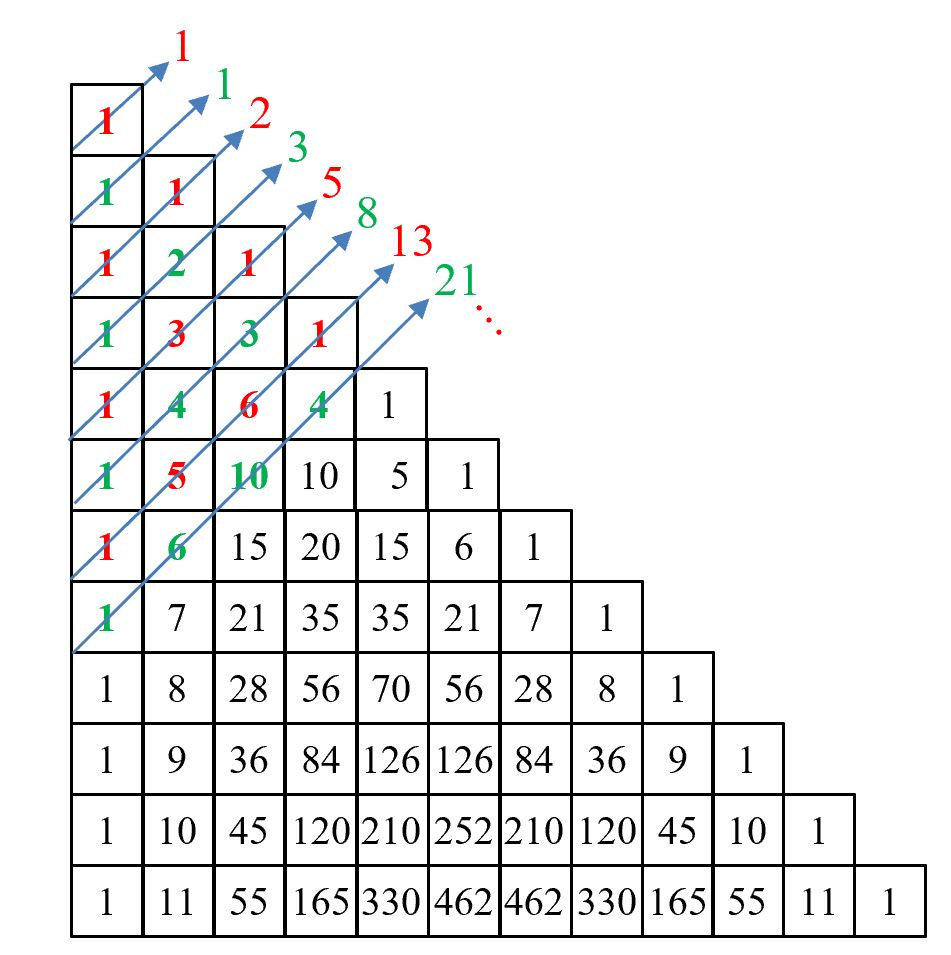
\includegraphics[width = 2 in]{Magazines/img/Vol4/pascal1.png}
\end{center}

When we sum the diagonals, we end up with the Fibonacci sequence! 

Remark: Written more formally, this fact is saying that
\[\sum_{k=0}^{\lfloor n/2\rfloor}\binom{n-k}k=F_{n+1}.\]
If you're comfortable with induction and summations, you might want to try proving this\footnote{Pascal's identity may be handy here.}!


\textbf{Sierpinski's triangle?!}

What happens when we color all the odd numbers in Pascal's triangle? It turns out, we get something that looks like Sierpinski's triangle! 

\begin{center}
	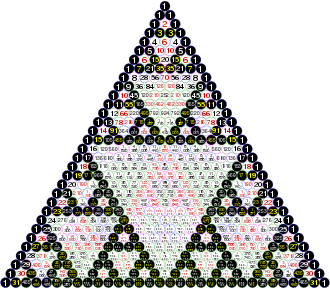
\includegraphics[scale=0.45]{Magazines/img/Vol4/pascal2.png}
\end{center}

And as we extend further and further downward, we get closer and closer to Sierpinski's triangle.

Things get even more interesting when we color every number based on their remainder when divided by different numbers. 

If we color based on their remainders when divided by $3$, $4$, and $5$, we get the following patterns. All of these images were taken from the \href{https://www.maa.org/press/periodicals/loci/joma/patterns-in-pascals-triangle-with-a-twist-first-twist-what-is-it}{MAA}:


\begin{center}
	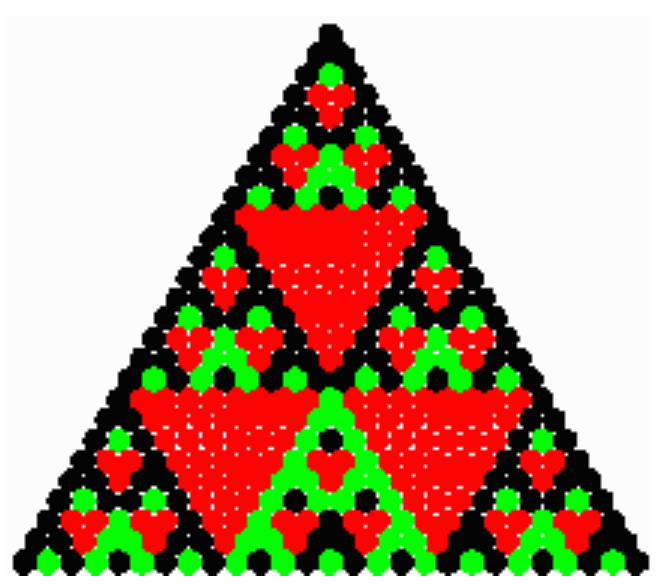
\includegraphics[scale=0.35]{Magazines/img/Vol4/pascal3.png}
\end{center}

\begin{center}
	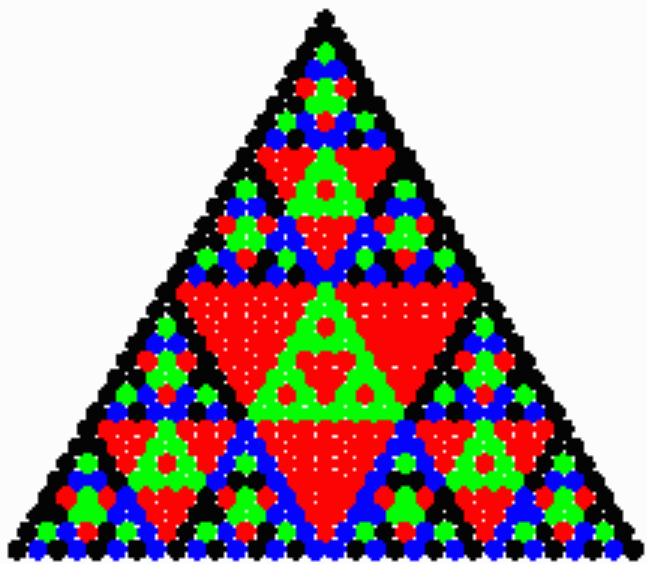
\includegraphics[scale=0.35]{Magazines/img/Vol4/pascal4.png}
\end{center}

\begin{center}
	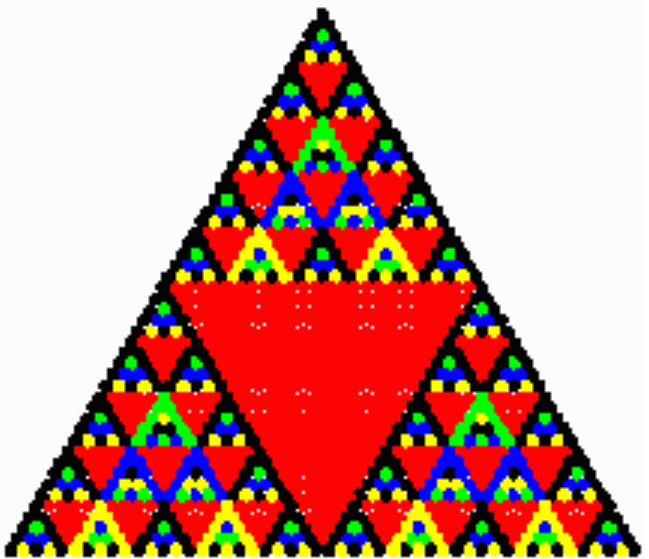
\includegraphics[scale=0.35]{Magazines/img/Vol4/pascal5.png}
\end{center}


Those were just some of the patterns in Pascal's popular triangle. Perhaps if you're patient, persistent, and play around a bit, you'll find even more!

\closearticle
\articletitle{The Strong Law of Small Numbers}{Michael Yang}{}
The number 31 is prime. You might have known that already; after all, it’s not too hard to check. But did you know that the number 331 is also prime? And 3331? Is this some mysterious pattern lurking in the prime numbers?
	
Sadly, the answer is no – after all, you’d probably already have heard about it if it were! But while this sequence doesn’t always produce prime numbers, it does go along for what some would say is an unreasonable amount of time. The first number in the sequence $3, 31, 331, …$ which is not prime is $333333331$, with eight threes at the beginning (it’s divisible by 17). Doesn’t it seem strange that such a quirky pattern would go on for so long?
	 
As it turns out, not really. Well, yes – it’s very interesting that this particular sequence produces so many primes. In the greater scope of things, however, it’s not out of character to see coincidences like this happen. This is just one example of the Strong Law of Small Numbers, a humorous proposition put forth by mathematician Richard Guy. 

\begin{center}
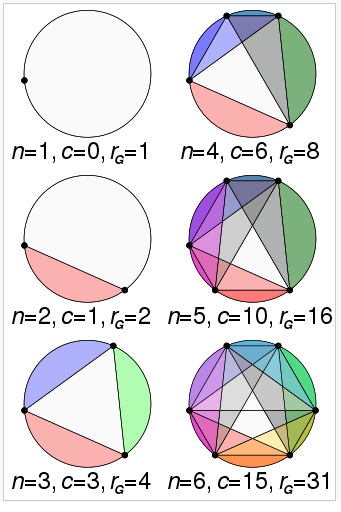
\includegraphics[scale=0.75]{Magazines/img/Vol4/strong_law_small_num.png}
\end{center}
 
Loosely, it states, “There aren’t enough small numbers to meet the many demands made of them.” Put another way, there are so many possible sequences generated in so many different ways that some of them will have to overlap for a while, even if they share no real connection with each other.
	
One of the most famous examples of this is the following function: Given a positive integer n, raise the number e (approximately $2.71828$) to the power of $(n – 1)/2$. Then, take the least integer above that number. As we do this for the first few positive integers, the numbers produced are $1, 2, 3, 5, 8, 13, 21, 34$, and $55$. Does this look familiar? These are precisely the numbers of the famed Fibonacci sequence! As it turns out, however, this magical Fibonacci generator fails after $55$: the next few terms are $91, 149,$ and $245$.

Another version of the Strong Law also shows up if you’ve ever had the fortune of hand-drawing complex geometry diagrams. Consider the following problem, which has recently made its way into mathematical lore:

Alice is practicing drawing triangles. She wants to draw an acute triangle whose angle measures are all multiples of $10$ (in degrees), is not isosceles, and has no $30-$ or $60-$ degree angles (to avoid some special coincidences). How many distinct triangles can Alice draw?
 
Taken one at a time, these are all very reasonable requests. But, if you do the working out, you’ll find that there are actually zero possible triangles that satisfy all of the criteria simultaneously! Alice is out of luck – a diagrammatic coincidence seems inevitable.

It’s important to note that while the Strong Law of Small Numbers is certainly present in many scenarios, it doesn’t reduce the power of conjecture and creativity in math. Sure, there are some seemingly-amazing patterns that chalk up to nothing more than a numerical coincidence. On the flip side, however, some of our greatest discoveries have also been uncovered via quantum leaps of faith. Just don’t jump to too many conclusions the next time you see a suspicious-looking pattern in a problem – as Guy puts it, “You can’t tell by looking.” 
\begin{center}
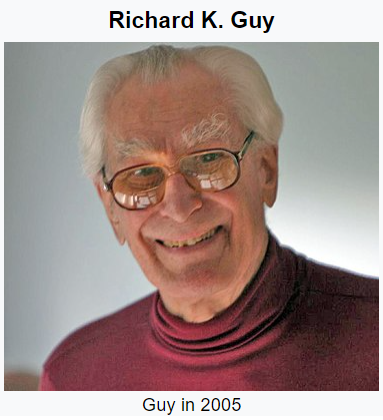
\includegraphics[scale=0.75]{Magazines/img/Vol4/richard_guy.png}
\end{center}

\closearticle
\articletitle{Arrow’s Impossibility Theorem}{Cecilia Sun}{}
\begin{center}
    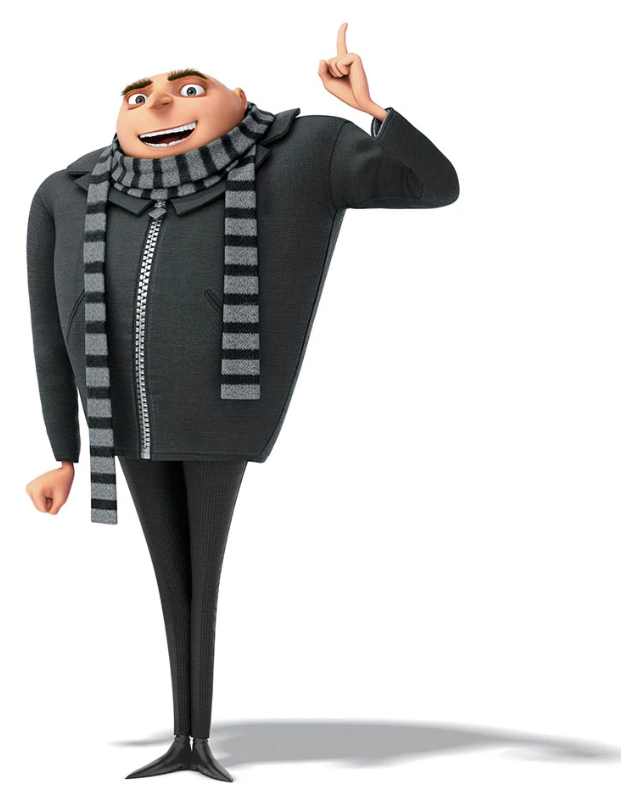
\includegraphics[scale=0.35]{Magazines/img/Vol4/gru.png}
\end{center}

Say you’re Gru of \textit{Despicable Me} fame, and you and your minions have just discovered a previously uninhabited island, on which you want to establish a new evil lab for you to conduct your evil experiments. Since you are Gru and must return home soon to be with Margo, Edith, and Agnes, your three adopted children, you have chosen a group of minions to stay on the island to do your evil bidding while you and the others return. However, the island minions soon run into an issue --- with you away from the island, who is going to be their leader? 

The minions suggest several voting schemes, and your job is to evaluate each of them and decide which one you want the minions to use:
\begin{itemize}
	\item \textbf{Stuart’s method}: Stuart is sensible, and proposes that each of the minions votes for one candidate. He will then count the number of votes each candidate has and use that to create a ranking of the candidates, and the minions will elect the candidate with the most votes.
	\item \textbf{Kevin’s method}: Kevin thinks the minions should take into account the second, third, etc. preferences of each individual minion. He proposes that they have each minion rank each of the $n$ candidates. For each ballot, the first choice candidate gets $n$ points, the second choice candidate gets $n-1$ points, etc. The candidates will be ranked based on their point total, and the minion with the greatest point total wins.
	\item \textbf{Bob’s method}: Bob is a dictator. Bob will rank all the candidates, and the minions will elect whoever Bob chooses as the winner. 
\end{itemize}

Ideally, want our voting systems to be \textit{fair} --- but what exactly does ``fair’’ mean? We might start with some criteria that will help us determine what a ``fair” system looks like:
\begin{itemize}
	\item \textbf{Universality}: We want our election system to be deterministic: in other words, there is no randomness involved in deciding who the winner is. Two identical sets of ballots should produce the same ranking and thus elect the same person every single time. 
	\item \textbf{Independence of irrelevant alternatives (IIA)}: The ranking between two candidates $x$ and $y$ should depend only on people’s preferences between $x$ and $y$; in other words, changes in individual voters’ preferences of any other candidate (say, $z$), should not impact the final ranking of $x$ and $y$ relative to each other. 
	For instance, if in the final ranking, Stuart is ranked higher than Kevin, then Stuart should be ranked higher than Kevin even if we disqualify Bob from the election. 
	
What happens when we don’t have IIA? Well, then there’s a potential for something like this to happen:
	%todo for cecilia: 
	%aroehus cropping is bad, i will fix later
	\begin{center}
	    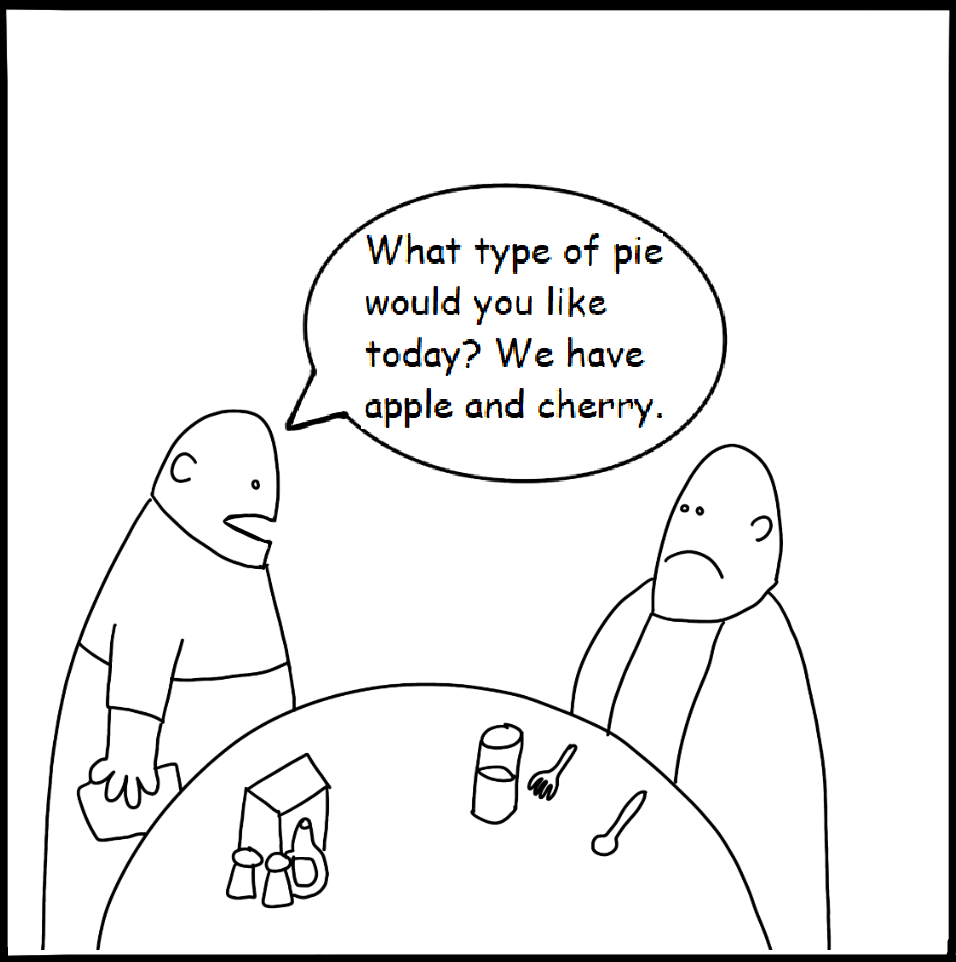
\includegraphics[width = \linewidth]{Magazines/img/Vol4/minions1.png}
	    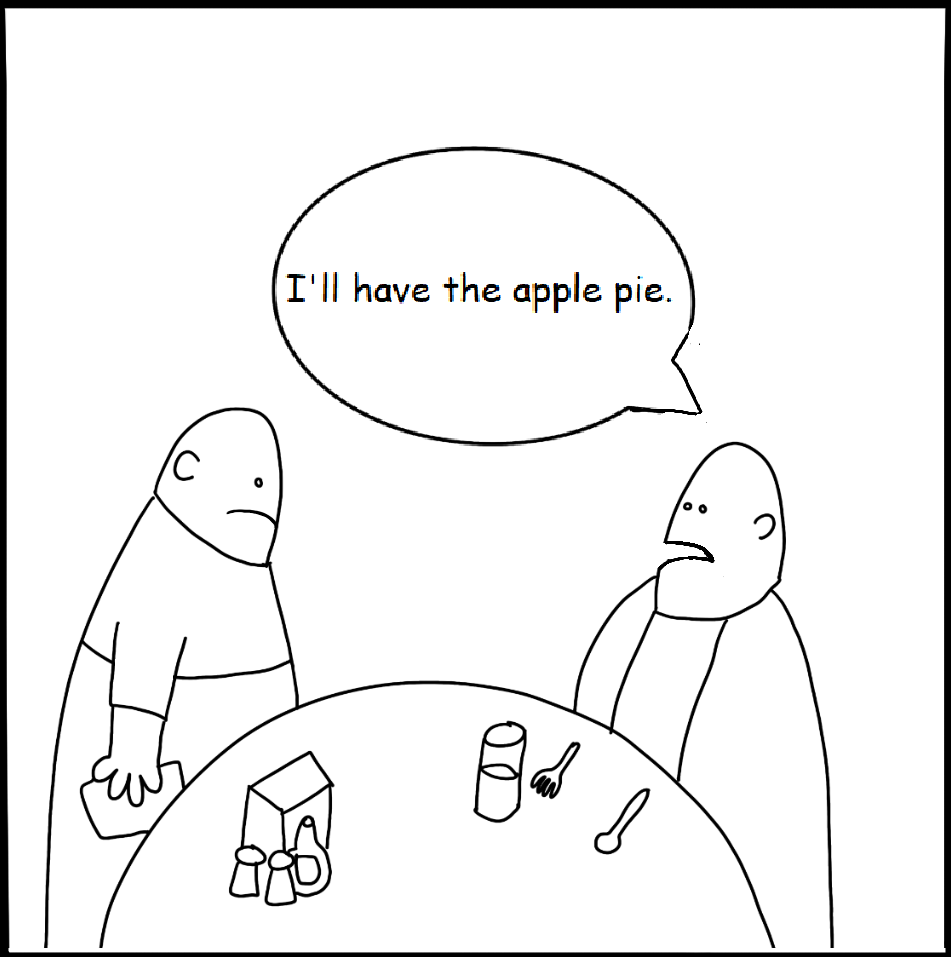
\includegraphics[width = \linewidth]{Magazines/img/Vol4/minions2.png}
	    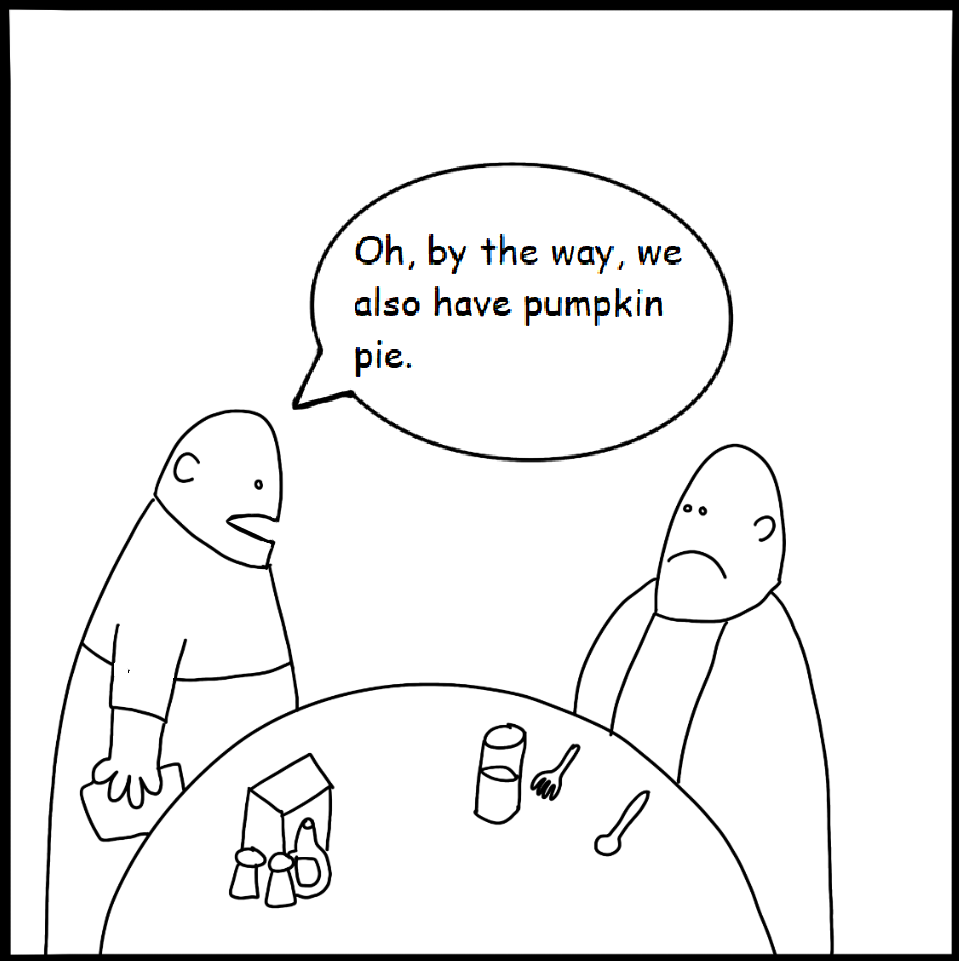
\includegraphics[width = \linewidth]{Magazines/img/Vol4/minions3.png}
	    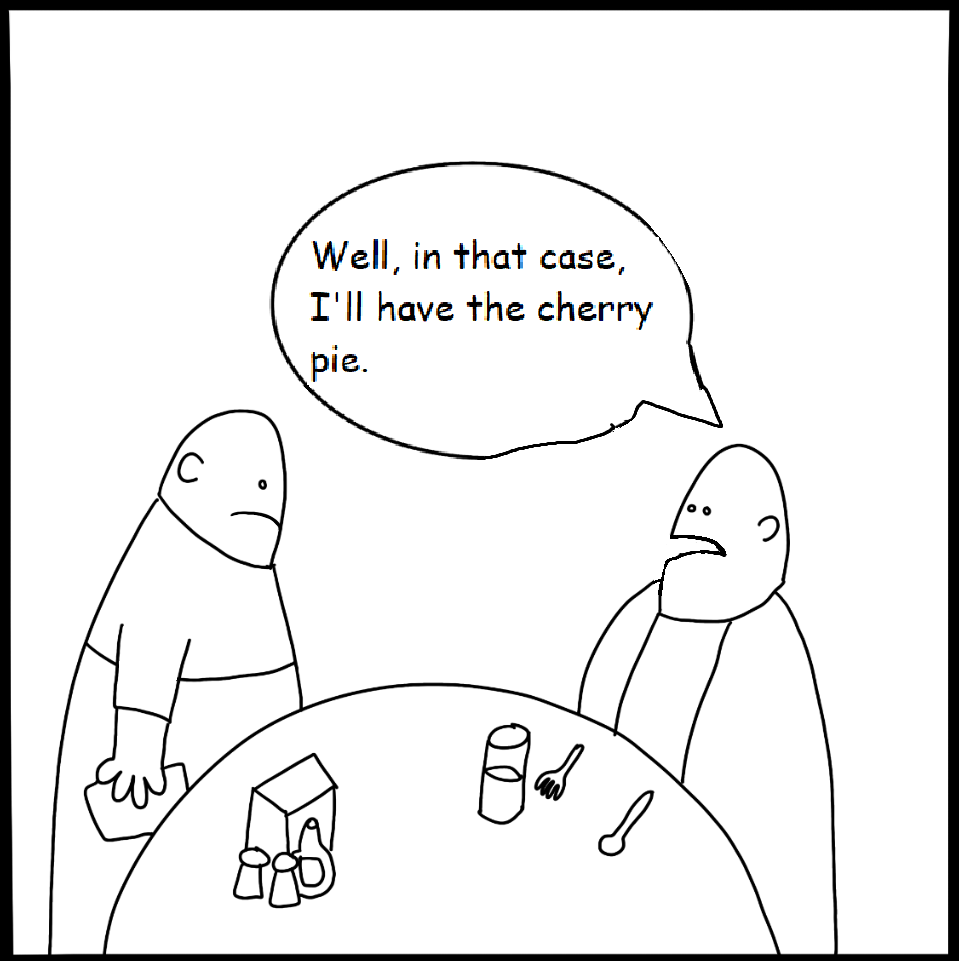
\includegraphics[width = \linewidth]{Magazines/img/Vol4/minions4.png}
	\end{center}
	
	
	\item \textbf{Monotonicity}: If an individual voter changes their vote by ranking one of the candidates higher, then the candidate’s position in the final ranking should either be higher or unchanged; in other words, a voter should not be able to hurt a candidate’s final ranking by ranking them higher. Similarly, a voter should not be able to boost a candidate’s final ranking by ranking them lower. 
	\item \textbf{Non-imposition}: It should be possible for any candidate to get elected! 
\end{itemize}

Let’s look at each of the three minions’ proposed strategies and evaluate their fairness based on our criteria:

\textbf{Stuart’s method}: Rank the candidates based on the number of first place votes they receive.
\begin{itemize}
	\item \textbf{Universality}: Stuart’s method {\textbf{satisfies}} universality: there is no randomness involved in his method.
	\item \textbf{IIA}: Stuart’s method {\textbf{violates}} IIA. Consider the following election between Stuart (S), Kevin (K), and Bob (B), where each column represents an individual voter’s ballot and the number of voters who had that ballot:
	\[
		\begin{array}{c|ccc}
				& 49 & 48 & 3 \\
			\text{1st} & S & K & B \\
			\text{2nd} & K & B & K \\
			\text{3rd} & B & S & S
		\end{array}
	\]

	Stuart wins this election, but if Bob is disqualified from the election, then the three votes for Bob will go to Kevin and he will then beat Stuart! 
	\item \textbf{Monotonicity}: Stuart’s method {\textbf{satisfies}} monotonicity: if a candidate has the most first-place votes, then giving them more first place votes will only put them higher in the ranking. 
	\item \textbf{Non-imposition}: Stuart method {\textbf{satisfies}} non-imposition: if all the minions rank a candidate first, then that candidate will win, and this is true of all candidates. 
\end{itemize}
Okay, so Stuart’s method is alright, but it does violate IIA, and in a pretty egregious fashion: in the example case, there are two candidates who are head to head and a third candidate who has very little support, which mimics a lot of real elections! 

\textbf{Kevin’s method}: For each ballot, give the first choice candidate $n$ points, the second choice gets $n-1$ points, etc. Then rank the candidates based on their point totals. 
\begin{itemize}
	\item \textbf{Universality}: Kevin’s method \textbf{satisfies} universality: there is no randomness involved in his method.
	\item \textbf{IIA}: Kevin’s method {\textbf{violates}} IIA. Consider the following election between Stuart (S), Kevin (K), Bob (B), and Dave (D):
	\[
		\begin{array}{c|ccc}
				& 14 & 8 & 4 \\
			\text{1st} & S & K & D \\
			\text{2nd} & K & D & S \\
			\text{3rd} & B & B & B \\
			\text{4th} & D & S & K
		\end{array}
	\]

	If we use Kevin’s method to determine the winner of this election, then Kevin wins with $78$ points. However, if we take Bob out of the election, then Stuart wins the election! 
	\item \textbf{Monotonicity}: Kevin’s method {\textbf{satisfies}} monotonicity: if a candidate has the most points, then ranking them higher will only increase their point count, and they can only move higher in the final ranking.
	\item \textbf{Non-imposition}: Kevin’s method {\textbf{satisfies}} non-imposition: if all the minions rank a candidate first, then that candidate will win, and this is true of all candidates. 
\end{itemize}
Even though Kevin’s method \textit{seems} to be more fair than Stuart's method, it still has the same IIA issues! 

\textbf{Bob’s method}: The ranking of candidates on Bob’s ballot is also the final ranking of candidates. 
\begin{itemize}
	\item \textbf{Universality}: Bob’s method {\textbf{satisfies}} universality: there is no randomness involved in his method.
	\item \textbf{IIA}: Bob’s method {\textbf{satisfies}} IIA! If a candidate drops out of the election, then the candidates’ placements relative to each other is the same since they are the same on Bob’s ballot, which is the only one that matters.
	\item \textbf{Monotonicity}: Bob’s method {\textbf{satisfies}} monotonicity. If a minion other than Bob changes their ballot, then all the candidates’ final placements remain the same, since Bob’s ballot is constant. If Bob changes his ballot to move a candidate higher, then the candidate will also be higher in the final ranking since the final ranking is determined by Bob’s ballot. 
	\item \textbf{Non-imposition}: Bob’s method {\textbf{satisfies}} non-imposition: if Bob ranks a candidate first, then that candidate wins, and this is true for all candidates
\end{itemize}

According to our criteria, Bob’s method is actually the fairest out of all the proposed methods! 

In 1950, economist Kenneth Arrow proved that, in fact, the only voting system that satisfies \textit{all} the fairness criteria is a dictatorship! 

This result may seem shocking, but its practicality has been questioned even by Arrow himself. Though there might exist extreme cases in which voting systems do things we don’t want them to do, if they, like Stuart and Kevin’s suggestions, are reasonable enough, then we can expect them to work enough of the time. ``Most systems are not going to work badly all of the time” said Arrow. ``All I proved is that all can work badly at times.”

\closearticle

\articletitle{Are You Rational?}{Edward Yu}{}
There is an old joke about Homo Economicus, a purely rational decision-making human that always seeks to maximize profit (to use fancy words, ``utility’’).
Of course, Homo Economicus is not Homo Sapiens, nor are we Mr. Spock; we are not purely logical beings all the time.
\begin{center}
    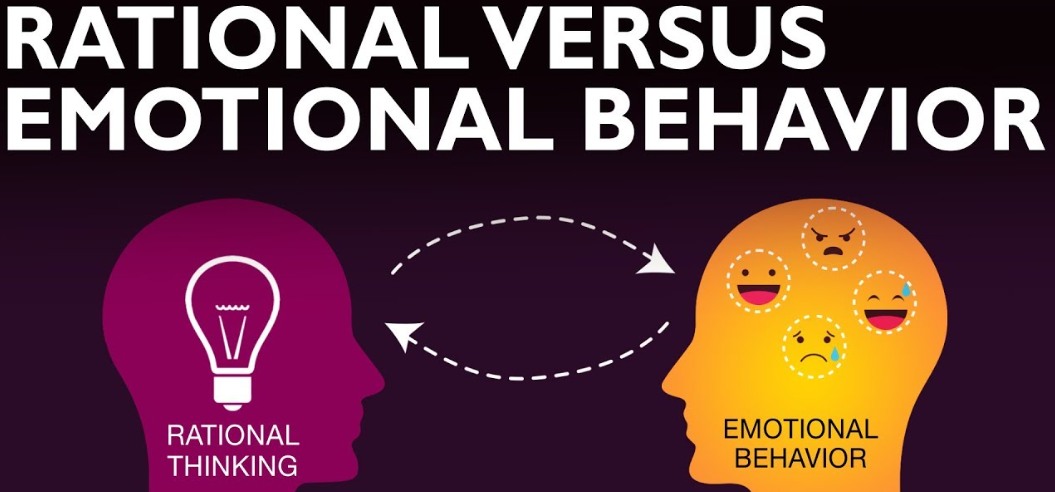
\includegraphics[scale=0.4]{Magazines/img/Vol4/rational.png}
\end{center}

We think we strive for logical decision-making during our most important decisions, yet we still are quite fallible. Here are some of my favorite examples of when human ``rational’’ decision-making goes awry.

\textbf{The Allais Paradox:} An eccentric billionaire offers you a choice between two gambles:
\begin{enumerate}
\item \$1 million, guaranteed, or
\item A 1\% chance of nothing, 89\% chance of getting \$1 million, and \$5 million otherwise?
\end{enumerate}
Most people choose the former over the latter: that 1\% chance of zero reward in the second scenario is intimidating, and perhaps not worth the (improbable) possibility of a \$5 million bonus.

Now, consider another choice. Would you rather take:
\begin{enumerate}
\item \$1 million with 11\% probability and nothing otherwise, or
\item \$5 million with 10\% probability and nothing otherwise?
\end{enumerate}
Once again, the decision is clear: there’s basically no distinction between 10\% and 11\%, and of course \$5 million is much more preferable to \$1 million, so we’ll go with the second choice.

The careful reader will already observe the problem: the two scenarios presented above are secretly the same scenario!
To get from the second scenario to the first one, the billionaire gives us an extra \$1 million with 89\% probability in both options. This paradoxically causes us to change our mind! It's as if we prefer apples to bananas, yet prefer an banana (plus a dollar bill) to an apple (plus a dollar bill).

So, why does the extra 1\% make such a difference? There are many formulations of the mathematically-reasoning human subconscious that seek to explain this away---``risk aversion'' and ``loss aversion'' are common related terms that you'll hear a lot on this context---but most of us are still faced with the gut-punch conclusion that we ``rationally'' made an inconsistent choice.

\textbf{The St. Petersburg Paradox:}
The eccentric billionaire is back! This time, they're going to play the following game with you. They throw in \$1 into the pot, and you repeatedly flip a coin. Every time the coin lands heads, the value of the pot doubles, and when the coin lands tails for the first time, you win everything in the pot.

\begin{center}
    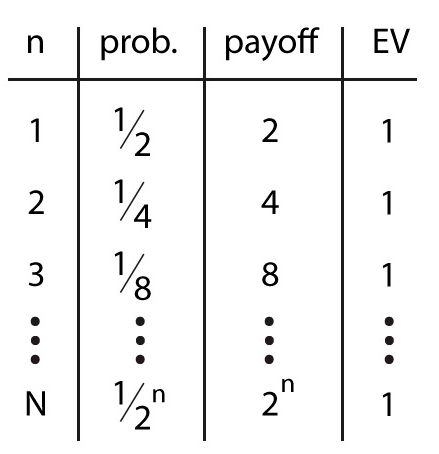
\includegraphics[scale=0.6]{Magazines/img/Vol4/st_petersberg.png}
\end{center}

So, for example, if you tossed three heads in a row followed by tails, you'd win \$8.
How much would you be willing to pay to play this game?

Supposedly, you should be willing to pay any amount of money: the expected payoff (your average winnings) is infinite! You can check this with a simple expected-value calculation:
\[1\times\frac12 + 2\times\frac14 + 4\times\frac18 + \cdots \]
\[= \frac12 + \frac12 + \frac12 + \cdots = \infty.\]

But before you sell all of your possessions to purchase a ticket (don't try this at home), keep in mind that the amount you'll win is probably vanishingly small: there's a 75\% chance you'll walk away with \$2 or less! So most of the value of the game comes from magnificently large payoffs with vanishingly small probabilities---in this case it's common sense that has to save us from the perils of expected-value-maximizing calculations.

\textbf{Newcomb’s Paradox:} The billionaire has one final challenge for you. They show you two boxes, labeled A and B, and you can choose to take either box B only, or both boxes A and B.
They also have an infallible crystal ball, which will predict your action.

You see the following in each box:
\begin{itemize}
    \item Box A is transparent and always contains a visible \$1,000.
    \item Box B is opaque (you can't see inside), but its content has been set by the predictor:
    \begin{itemize}
    \item If the predictor has predicted that the player will take both boxes A and B, then box B contains nothing.
    \item If the predictor has predicted that the player will take only box B, then box B contains \$1,000,000.
    \end{itemize}
\end{itemize}
Should you take B only (known as ``one-boxing''), or both A and B (known as ``two-boxing'')?

It has been remarked that to almost everyone, it is perfectly obvious what should be done, but ``the difficulty is that these people seem to divide almost evenly on the problem, with large numbers thinking that the opposing half is just being silly.''
I'll leave the analysis of this last one to you, since philosophers even today are divided on which option to take. Enjoy---and remember, always, that you might not always be thinking rationally!
\closearticle

\begin{center}
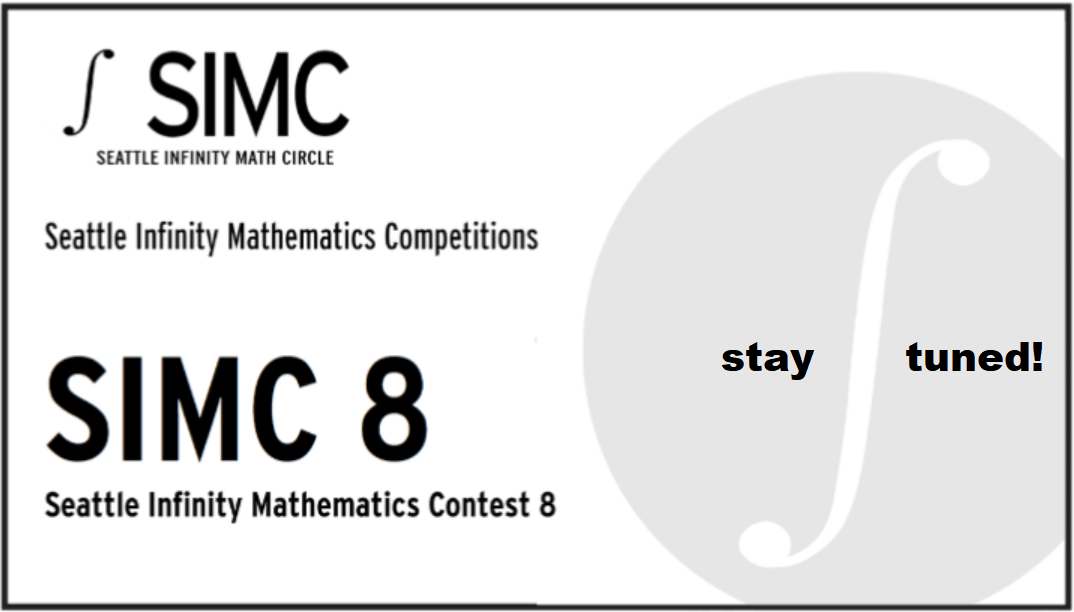
\includegraphics[scale=0.2]{Magazines/img/Vol4/simc8.png} 

\href{https://docs.google.com/forms/d/e/1FAIpQLScB4ig6bxgUfaDa0i6csRy8Wmn3a3ezEV81MeVDZOp4wKVNTA/viewform}{Register for the SIMC 8 here!}
\end{center}

\vspace{1.0cm}
\begin{tabular}{c l}
  
\includegraphics[scale=0.06,valign=c]{Magazines/img/email.png}
    & \href{mailto:seattleinfinitymathcircle@gmail.com}{Email}\\
  \;\\
  
\includegraphics[scale=0.1,valign=c]{Magazines/img/website.png}
    & \href{https://seattleinfinity.org}{Website} \\
  
\includegraphics[scale=0.5,valign=c]{Magazines/img/facebook.png}
    & \href{https://www.facebook.com/simathcircle/}{Facebook} \\
  
\includegraphics[scale=0.5,valign=c]{Magazines/img/insta.png}
    & \href{https://www.instagram.com/seattleinfinitymathcircle/}{Instagram} \\
  
\includegraphics[scale=0.5,valign=c]{Magazines/img/youtube.png}
    & \href{https://www.youtube.com/channel/UCgwA-iysWPc_XG0R0AZ5z5g/videos}{YouTube} \\
  
\includegraphics[scale=0.013,valign=c]{Magazines/img/discord.png}
    & \href{https://discord.gg/2Ma3dURhTt}{Discord} 
\end{tabular}

\end{multicols}

\end{document}
